% This file was converted to LaTeX by Writer2LaTeX ver. 1.0.2
% see http://writer2latex.sourceforge.net for more info
\documentclass[12pt]{article}
\usepackage[utf8]{inputenc}
\usepackage[T1]{fontenc}
\usepackage[english]{babel}
\usepackage{amsmath}
\usepackage{amssymb,amsfonts,textcomp}
\usepackage{array}
\usepackage{supertabular}
\usepackage{hhline}
\usepackage{hyperref}
\hypersetup{colorlinks=true, linkcolor=blue, citecolor=blue, filecolor=blue, urlcolor=blue}
\usepackage{graphicx}
\newcommand\textsubscript[1]{\ensuremath{{}_{\text{#1}}}}
% Text styles
\newcommand\textstylespellingerror[1]{#1}
\makeatletter
\newcommand\arraybslash{\let\\\@arraycr}
\makeatother
\raggedbottom
% Paragraph styles
\renewcommand\familydefault{\rmdefault}
\newenvironment{styleStandard}{\setlength\leftskip{0cm}\setlength\rightskip{0cm plus 1fil}\setlength\parindent{0cm}\setlength\parfillskip{0pt plus 1fil}\setlength\parskip{0in plus 1pt}\writerlistparindent\writerlistleftskip\leavevmode\normalfont\normalsize\writerlistlabel\ignorespaces}{\unskip\vspace{0.111in plus 0.0111in}\par}
\newenvironment{stylelsAbstract}{\setlength\leftskip{0.5in}\setlength\rightskip{0.5in}\setlength\parindent{0in}\setlength\parfillskip{0pt plus 1fil}\setlength\parskip{0in plus 1pt}\writerlistparindent\writerlistleftskip\leavevmode\normalfont\normalsize\itshape\writerlistlabel\ignorespaces}{\unskip\vspace{0.111in plus 0.0111in}\par}
\newenvironment{stylelsSectioni}{\setlength\leftskip{0.25in}\setlength\rightskip{0in plus 1fil}\setlength\parindent{0in}\setlength\parfillskip{0pt plus 1fil}\setlength\parskip{0.1665in plus 0.016649999in}\writerlistparindent\writerlistleftskip\leavevmode\normalfont\normalsize\fontsize{18pt}{21.6pt}\selectfont\bfseries\writerlistlabel\ignorespaces}{\unskip\vspace{0.0835in plus 0.00835in}\par}
\newenvironment{stylelsEnumerated}{\renewcommand\baselinestretch{1.0}\setlength\leftskip{0cm}\setlength\rightskip{0cm plus 1fil}\setlength\parindent{0cm}\setlength\parfillskip{0pt plus 1fil}\setlength\parskip{0in plus 1pt}\writerlistparindent\writerlistleftskip\leavevmode\normalfont\normalsize\writerlistlabel\ignorespaces}{\unskip\vspace{0.0972in plus 0.00972in}\par}
\newenvironment{stylelsSectionii}{\setlength\leftskip{0.25in}\setlength\rightskip{0in plus 1fil}\setlength\parindent{0in}\setlength\parfillskip{0pt plus 1fil}\setlength\parskip{0.222in plus 0.0222in}\writerlistparindent\writerlistleftskip\leavevmode\normalfont\normalsize\fontsize{16pt}{19.2pt}\selectfont\bfseries\writerlistlabel\ignorespaces}{\unskip\vspace{0.0835in plus 0.00835in}\par}
\newenvironment{stylelsSectioniii}{\setlength\leftskip{0.5717in}\setlength\rightskip{0in plus 1fil}\setlength\parindent{0in}\setlength\parfillskip{0pt plus 1fil}\setlength\parskip{0.0972in plus 0.00972in}\writerlistparindent\writerlistleftskip\leavevmode\normalfont\normalsize\fontsize{14pt}{16.8pt}\selectfont\bfseries\writerlistlabel\ignorespaces}{\unskip\vspace{0in plus 1pt}\par}
% List styles
\newcommand\writerlistleftskip{}
\newcommand\writerlistparindent{}
\newcommand\writerlistlabel{}
\newcommand\writerlistremovelabel{\aftergroup\let\aftergroup\writerlistparindent\aftergroup\relax\aftergroup\let\aftergroup\writerlistlabel\aftergroup\relax}
\newcounter{listWWNumxxiileveli}
\newcounter{listWWNumxxiilevelii}[listWWNumxxiileveli]
\newcounter{listWWNumxxiileveliii}[listWWNumxxiilevelii]
\newcounter{listWWNumxxiileveliv}[listWWNumxxiileveliii]
\renewcommand\thelistWWNumxxiileveli{\arabic{listWWNumxxiileveli}}
\renewcommand\thelistWWNumxxiilevelii{\arabic{listWWNumxxiileveli}.\arabic{listWWNumxxiilevelii}}
\renewcommand\thelistWWNumxxiileveliii{\arabic{listWWNumxxiileveli}.\arabic{listWWNumxxiilevelii}.\arabic{listWWNumxxiileveliii}}
\renewcommand\thelistWWNumxxiileveliv{\arabic{listWWNumxxiileveli}.\arabic{listWWNumxxiilevelii}.\arabic{listWWNumxxiileveliii}.\arabic{listWWNumxxiileveliv}}
\newcommand\labellistWWNumxxiileveli{\thelistWWNumxxiileveli.}
\newcommand\labellistWWNumxxiilevelii{\thelistWWNumxxiilevelii.}
\newcommand\labellistWWNumxxiileveliii{\thelistWWNumxxiileveliii.}
\newcommand\labellistWWNumxxiileveliv{\thelistWWNumxxiileveliv.}
\newenvironment{listWWNumxxiileveli}{\def\writerlistleftskip{\addtolength\leftskip{0.0cm}}\def\writerlistparindent{}\def\writerlistlabel{}\def\item{\def\writerlistparindent{\setlength\parindent{-0cm}}\def\writerlistlabel{\stepcounter{listWWNumxxiileveli}\makebox[0cm][l]{\labellistWWNumxxiileveli}\hspace{0cm}\writerlistremovelabel}}}{}
\newenvironment{listWWNumxxiilevelii}{\def\writerlistleftskip{\addtolength\leftskip{0.0cm}}\def\writerlistparindent{}\def\writerlistlabel{}\def\item{\def\writerlistparindent{\setlength\parindent{-0cm}}\def\writerlistlabel{\stepcounter{listWWNumxxiilevelii}\makebox[0cm][l]{\labellistWWNumxxiilevelii}\hspace{0cm}\writerlistremovelabel}}}{}
\newenvironment{listWWNumxxiileveliii}{\def\writerlistleftskip{\addtolength\leftskip{0.0cm}}\def\writerlistparindent{}\def\writerlistlabel{}\def\item{\def\writerlistparindent{\setlength\parindent{-0cm}}\def\writerlistlabel{\stepcounter{listWWNumxxiileveliii}\makebox[0cm][r]{\labellistWWNumxxiileveliii}\hspace{0cm}\writerlistremovelabel}}}{}
\newenvironment{listWWNumxxiileveliv}{\def\writerlistleftskip{\addtolength\leftskip{0.0cm}}\def\writerlistparindent{}\def\writerlistlabel{}\def\item{\def\writerlistparindent{\setlength\parindent{-0cm}}\def\writerlistlabel{\stepcounter{listWWNumxxiileveliv}\makebox[0cm][l]{\labellistWWNumxxiileveliv}\hspace{0cm}\writerlistremovelabel}}}{}
\newcounter{listWWNumxleveli}
\newcounter{listWWNumxlevelii}[listWWNumxleveli]
\newcounter{listWWNumxleveliii}[listWWNumxlevelii]
\newcounter{listWWNumxleveliv}[listWWNumxleveliii]
\renewcommand\thelistWWNumxleveli{\arabic{listWWNumxleveli}}
\renewcommand\thelistWWNumxlevelii{\alph{listWWNumxlevelii}}
\renewcommand\thelistWWNumxleveliii{\roman{listWWNumxleveliii}}
\renewcommand\thelistWWNumxleveliv{\arabic{listWWNumxleveliv}}
\newcommand\labellistWWNumxleveli{\thelistWWNumxleveli.}
\newcommand\labellistWWNumxlevelii{\thelistWWNumxlevelii.}
\newcommand\labellistWWNumxleveliii{\thelistWWNumxleveliii.}
\newcommand\labellistWWNumxleveliv{\thelistWWNumxleveliv.}
\newenvironment{listWWNumxleveli}{\def\writerlistleftskip{\addtolength\leftskip{0.0cm}}\def\writerlistparindent{}\def\writerlistlabel{}\def\item{\def\writerlistparindent{\setlength\parindent{-0cm}}\def\writerlistlabel{\stepcounter{listWWNumxleveli}\makebox[0cm][l]{\labellistWWNumxleveli}\hspace{0cm}\writerlistremovelabel}}}{}
\newenvironment{listWWNumxlevelii}{\def\writerlistleftskip{\addtolength\leftskip{0.0cm}}\def\writerlistparindent{}\def\writerlistlabel{}\def\item{\def\writerlistparindent{\setlength\parindent{-0cm}}\def\writerlistlabel{\stepcounter{listWWNumxlevelii}\makebox[0cm][l]{\labellistWWNumxlevelii}\hspace{0cm}\writerlistremovelabel}}}{}
\newenvironment{listWWNumxleveliii}{\def\writerlistleftskip{\addtolength\leftskip{0.0cm}}\def\writerlistparindent{}\def\writerlistlabel{}\def\item{\def\writerlistparindent{\setlength\parindent{-0cm}}\def\writerlistlabel{\stepcounter{listWWNumxleveliii}\makebox[0cm][r]{\labellistWWNumxleveliii}\hspace{0cm}\writerlistremovelabel}}}{}
\newenvironment{listWWNumxleveliv}{\def\writerlistleftskip{\addtolength\leftskip{0.0cm}}\def\writerlistparindent{}\def\writerlistlabel{}\def\item{\def\writerlistparindent{\setlength\parindent{-0cm}}\def\writerlistlabel{\stepcounter{listWWNumxleveliv}\makebox[0cm][l]{\labellistWWNumxleveliv}\hspace{0cm}\writerlistremovelabel}}}{}
\setlength\tabcolsep{1mm}
\renewcommand\arraystretch{1.3}
% footnotes configuration
\makeatletter
\renewcommand\thefootnote{\arabic{footnote}}
\makeatother
\title{}
\author{Jennifer Ament}
\date{2018-03-01}
\begin{document}
\title{\textsuperscript{Teachers’ assessment of perceived foreign accent and comprehensibility in adolescent EFL oral production in Study Abroad and F}ormal Instruction contexts: a mixed-method study}
\maketitle

\begin{styleStandard}
\textstylespellingerror{Carmen del Río, Maria Juan-Garau, Carmen Pérez-Vidal}
\end{styleStandard}

\begin{stylelsAbstract}
Research on second language acquisition has long been interested in analyzing different learning contexts that language learners experience when trying to improve their target languages (Collentine \& Freed 2004) such as formal instruction (FI), study abroad (SA), and, more recently, different types of immersion (Perez-Vidal 2017). The aim of the present study is to examine two of these contexts, SA and FI at home, in the case of English as a foreign language adolescent learners having Catalan and Spanish as their first languages, an age band which has received comparatively less attention than others (but see Llanes 2012; Llanes \& Muñoz 2013). We focus on the learners’ foreign accent and comprehensibility, as judged by a group of non-native listeners, with the objective of assessing progress and the relationship between both dimensions, following Trofimovich \& Isaacs (2012). Most centrally, we are interested in analyzing the aspects of each speech dimension on focus which have reportedly affected the judges’ ratings. In order to do that, speech samples were collected longitudinally for the SA (N = 25) and the FI (N = 31) groups of learners, respectively, with a pre-test/post-test design. Listeners were asked to rate and report on the aspects which affected their ratings. Our results reveal that the aspect which most influenced the judges was pronunciation. This places pronunciation at the center of the search for better practices in instructed second language acquisition in line with recently published studies (Van Loon 2002; Darcy, Ewert \& Lidster 2012; Gordon \& Darcy 2012; Saito \& Lyster 2012; Grant 2014).
\end{stylelsAbstract}

\setcounter{listWWNumxxiileveli}{0}
\begin{listWWNumxxiileveli}
\item 
\begin{stylelsSectioni}
Introduction
\end{stylelsSectioni}

\end{listWWNumxxiileveli}
\begin{styleStandard}
Within the communicative approach to language teaching, many second language (L2) researchers and teachers would agree that intelligibility is the main aim in oral communication and L2 pronunciation instruction, rather than a native-like accent. Indeed, the main objective of L2 learners in most cases is to be able to communicate and be understood, rather than accent reduction (Pennington \& Richards 1986; Derwing \& Munro 1997; Jenkins 2000; Munro 2008). The abilities linked to communication have been described on the basis of two constructs, intelligibility and comprehensibility. In previous studies a distinction between these two has been made (Munro \& Derwing 1995; 1999; Derwing \& Munro 1997; 2009). Intelligibility has been defined as the extent to which a given utterance is understood by a listener, and comprehensibility has been used to refer to the listeners’ own perception of how easily they understand an utterance. However, in the present study, we have chosen the term ‘comprehensibility’ to refer to the construct which some studies have identified as ‘intelligibility’, in line with Isaacs \& Trofimovich (2012). \ 
\end{styleStandard}

\begin{styleStandard}
All in all, both in authentic communication and in the interaction which takes place with teachers in classrooms, accentedness may play a role which, to some extent, may eventually account for the felicitious accomplishment of interactions. This is the focus of our study, which seeks to disentagle the issue of the degree to which speech accentedness may count more than comprehensibility when teachers evaluate learners. More specifically, we first want to exame the correlation between these two speech dimensions based on the ratings provided by the teachers/listeners in our study \ in relation to the pronunciation of two groups of English as a foreign language (EFL) adolescent learners: one group experiencing a 3-month study abroad (SA) programme, and another group experiencing conventional formal instruction in the at home (AH) institution. In a previous research study (del Río 2013) we compared gains in those two dimensions by each group respectively. Results indicated that SA participants obtained significantly greater gains in FA than the AH group. The findings also suggested that the SA context was more beneficial than the AH context in terms of comprehensibility development, since the percentage of learners improving their comprehensibility scores during SA was significantly larger than the percentage of learners improving their scores in the AH context, and SA learners obtained larger comprehensibility gains than AH learners, although such improvement was not significant (see Del Rio,2013: 139-164 ). Second, we want to explore the aspects which listeners consider when evaluating foreign accent and comprehensibility in SA learners’ speech samples when completing a perception task. We aim at identifying and drawing comparisons across the different factors underlying the judges’ accentedness and comprehensibility ratings (following the analyses conducted by Trofimovich \& Isaacs 2012). \ As pointed out by Isaacs (2010), knowledge of the factors influencing comprehensibility in L2 speech can help teachers to set instructional objectives, integrate pronunciation with the teaching of other skills, and take these questions into account in their assessment practice in the EFL classroom, and when preparing learners for SA experiences.
\end{styleStandard}

\begin{listWWNumxxiileveli}
\item 
\begin{stylelsSectioni}
Literature review
\end{stylelsSectioni}

\end{listWWNumxxiileveli}
\begin{styleStandard}
Two main principles have traditionally led the discussion about the objectives of pronunciation instruction: the \textit{nativeness principle} versus the \textit{intelligibility principle} (Levis 2005), i.e. comprehensibility. The \textit{nativeness principle} aims at native-like pronunciation for L2 speakers, whereas the \textit{intelligibility principle} considers intelligibility. , That is, how easily messages can be understood (what we refer as comprehensibility in this article)as the primary objective. 
\end{styleStandard}

\begin{styleStandard}
Following the latter principle, most L2 pronunciation research does not consider accent reduction to be the goal for communicative teaching and claims that pronunciation teaching should aim at language intelligibility (Kenworthy 1987; Pennington 1996; Derwing 2008; Thomson 2013). Thus, the interest when teaching pronunciation is not centred on the nuances of particular speech sounds, but on getting the L2 learners up to a level of competence which should allow them to deal with everyday communication situations (Gimson 1994). 
\end{styleStandard}

\begin{styleStandard}
In this study we have chosen to adopt the construt of ‘intelligibility’ and not that of nativelikeness \ in line with Isaacs \& Trofimovich (2012), who adopted Levis’ (2006) distinction between broad and narrow definitions of intelligibility. In its narrow sense, intelligibility refers to listeners’ actual understanding of L2 speech (Munro \& Derwing 1999). It is often measured by examining listeners’ accuracy in providing orthographic transcriptions of L2 speech, although other methods have also been used (e.g. comprehension questions, true-false statements, reaction times). In its broad sense, intelligibility is defined as listeners’ ability to understand speech. 
\end{styleStandard}

\begin{styleStandard}
However, the story does not end here, as two other concepts have also been the focus of attention when discussing pronunciation in formal instruction: \textit{foreign accent} and \textit{comprehensibility}. \ The former reflects how far from target-like standards learners’ speech is, the latter, how easy it is for listeners to perceive the information contained in learners’ messages (Isaacs 2010). As far as accentedness is concerned, we understand this concept as the listeners’ perception of how closely the pronunciation of an L2 utterance resembles that of a NS of English (Munro \& Derwing 1995; 1999; Derwing \& Munro 1997; 2009). Although L2 learners do not necessarily consider having a native-like pronunciation as a priority, there might be L2 learners who aim at achieving it for different reasons (e.g. professional reasons, building up a certain ‘self-image’, integrative motivation, etc.). In contrast, we may find L2 learners preferring to retain something of their first language (L1) accent when speaking in an additional language (Porter \& Garvin 1989). Dalton \& Seidlhofer (1994: 7) note that “pronunciation is so much a matter of self-image that students may prefer to keep their accent deliberately, in order to retain their self-respect or to gain the approval of their peers.” This is indeed what we often find as teachers in the foreign language classroom when our students tend to avoid sounding ‘English’, since this can result in their peers joking about their ‘native like accent’ (Fisher \& Evans 2000). As for comprehensibility, according to Levis (2006: 252), intelligibility “is not usually distinguished from closely related terms such as comprehensibility” and has been typically measured through listeners’ ratings of how easily they understand speech (Munro \& Derwing 1999). As Isaacs \& Trofimovich (2012) pointed out, it is actually comprehensibility (not intelligibility) that is being assessed when listeners rate how easily they understand the information contained in a message. Therefore, in line with Trofimovich \& Isaacs (2012), in this study, instead of intelligibility, we have adopted the construct of comprehensibility, which falls under Levis’ broad sense of intelligibility and reflects a common approach to assessing intelligibility in oral proficiency scales.
\end{styleStandard}

\begin{styleStandard}
Finally, and most importantly for this study, \ it must be pointed out that the two constructs, foreign accent and comprehensibility, have been claimed to constitute two partially independent dimensions. Regrettably, this may not be reflected in some assessment rubrics and actual assessment practices, which very often conflate these two different, albeit partially overlapping, dimensions of speech production. As Munro \& Derwing (1995: 92) note, we may find pronunciation assessment scales ranging from “not accented, perfectly comprehensible at one endpoint to accented and difficult to understand at the other.” Given the possible overlap between different dimensions in popular assessment practices, our research study precisely aims at analyzing whether teachers are aware of these two different constructs currently included in the analysis of speech production. In other words, the aim of this study is to examine the extent to which teachers bear in mind the distinction between foreign accent and comprehensibility when they rate their learners’ speech productions.
\end{styleStandard}

\begin{styleStandard}
In this respect, results reported by previous studies examining the relationship between foreign accent and comprehensibility posit that heavily accented speech can often be perfectly understood (Munro \& Derwing 1995; 1999; Derwing \& Munro 1997; Gallardo del Puerto et al. 2007; Munro 2008; Hayes-Harb \& Watzinger-Tharp 2012). Producing comprehensible speech is more than a matter of pronunciation. While it is true that some errors in pronunciation may affect speech comprehensibility, foreign-accented speech does not necessarily impede comprehensibility. Thus, if comprehensibility is the main objective of pronunciation instruction, the degree of foreign accent in L2 learners’ oral productions should be of minor concern, and accent reduction should not be a priority. Rather, those aspects of L2 speech that appear to interfere with listeners’ comprehension of the learners’ production should be the focus. The question is: which aspects do seem to affect comprehensibility? 
\end{styleStandard}

\begin{styleStandard}
A research priority is to distinguish the aspects of L2 speech that hinder comprehensibility from those that, while noticeable or irritating, do not impede understanding the message (Munro 2008; Isaacs \& Trofimovich 2012). Little empirical research has examined the particular aspects of foreign-accented speech which affect comprehensibility (Munro \& Derwing 1995; 1999; Zielinski 2008; Isaacs \& Trofimovich 2012; Trofimovich \& Isaacs 2012). Moreover, opinions of a particular L2 speaker’s pronunciation problems may vary from listener to listener since familiarity with accented speech and individual differences in the ability to comprehend L2 speech may influence foreign accent and comprehensibility perception (Gass \& Varonis 1984; Munro \& Derwing 1999). 
\end{styleStandard}

\begin{styleStandard}
In line with Derwing \& Munro (2009), we believe it is appropriate to work on those aspects of accent which may affect comprehensibility. Some studies have indicated that pronunciation training can help L2 speakers produce more comprehensible speech. Derwing et al. (1998) examined perceived accentedness, comprehensibility and fluency in the oral productions of L2 learners of English. The learners were assigned to one of these conditions: (1) no specific pronunciation instruction group; (2) global instruction group, who received instruction with a focus on features such as speaking rate, intonation, rhythm, projection, word stress, and sentence stress; and (3) segmental instruction group, who received instruction to improve their production of individual sounds. Their research concluded that even though the two groups receiving instruction in pronunciation showed significant improvement in accentedness and comprehensibility on the sentences, only the group receiving global instruction showed improvement in comprehensibility and fluency in the narratives. 
\end{styleStandard}

\begin{styleStandard}
In line with these results, Munro \& Derwing (1999: 285) reported that “prosodic errors appear to be a more potent force in the loss of intelligibility than phonetic errors.” These findings are in opposition with the actual situation in the EFL classroom, where much pronunciation practice and error correction focuses on the segmental level.
\end{styleStandard}

\begin{styleStandard}
More recently, Trofimovich \& Isaacs (2012) and Isaacs \& Trofimovich (2012) explored the linguistic aspects which affect foreign accent and comprehensibility. In the former study, Trofimovich \& Isaacs (2012) examined the linguistic aspects of L2 speech related to accent and comprehensibility. They concluded that both dimensions were related to many speech measures, but that “four categories uniquely distinguished accent from comprehensibility, with all categories specific to the dimension of phonology (i.e. vowels and consonants, syllables, sounding nativelike, and rhythm)”, whereas comprehensibility was additionally linked to grammatical accuracy and lexical richness. Although it is true that speaking involves pronunciation, it is worth highlighting that L2 speech comprehensibility was found to be linked to vocabulary and grammar. In the second study, Isaacs \& Trofimovich (2012) studied the construct of comprehensibility in greater depth, and explored the aspects of speech that affected L2 comprehensibility at different ability levels. Based on the analyses of 19 quantitative speech measures, and listeners’ judgments and introspective reports, the authors identified five speech measures that distinguished between L2 learners at different comprehensibility levels: “lexical richness and fluency measures differentiated between low-level learners; grammatical and discourse-level measures differentiated between high-level learners; and word stress errors discriminated between learners of all levels” (Isaacs \& Trofimovich 2012: 476). Thus, it is interesting to highlight that not only pronunciation features of foreign-accented speech, but also other language aspects affect speech comprehensibility (e.g. vocabulary, grammar, and discourse measures). 
\end{styleStandard}

\begin{styleStandard}
The studies mentioned above included English native speakers (NSs) as listeners of L2 learners’ oral production. It has been claimed that work on perceived accentedness and comprehensibility with non-native listeners is still insufficient (Derwing \& Munro 2011; Isaacs \& Trofimovich 2012). What for example some of these studies have suggested is the possibility of a speech comprehensibility benefit in those situations where non-native speakers (NNSs) and listeners share the same L1 background (Gallardo del Puerto et al. 2007). However, further evidence is necessary to strengthen this argument. Thus, the present study provides data regarding perceived foreign accent and comprehensibility, with data from a group of adolescent EFL learners who have experienced a period of residence in the target language country (United Kingdom) and formal instruction (FI) in their home country, Spain, and from a group of Spanish L1 non-native listeners, who are EFL teachers, allowing for comparisons with previous studies including native listeners to be made to see if our results agree with previous findings. 
\end{styleStandard}

\begin{styleStandard}
Cocnerning the specific focus of the current study, there is a bulk of research \ focusing on accentedness and comprehensibility with a similar population, namely EFL FI learners in Spain, sometimes contrasting them with Content and Language Integrated Learning (CLIL) learners (García Lecumberri \& Gallardo del Puerto 2003; Gallardo del Puerto et al. 2007; Rallo \& Juan-Garau 2011). However, to our knowledge, none of them has included a group participating in a SA context of learning, and examined the possible differences which may result (but see Llanes 2012; Llanes \& Muñoz 2012). In sum, no previous study exists focusing on the issues of accentedness and comprehensibility, from the perspective of the raters, in the case of adolescent SA EFL learners.
\end{styleStandard}

\begin{listWWNumxxiileveli}
\item 
\begin{stylelsSectioni}
The present study
\end{stylelsSectioni}

\end{listWWNumxxiileveli}
\begin{styleStandard}
The current study aims at probing the constructs of foreign accent and comprehensibility as understood and used by listeners when asked to rate EFL learners’ speech production. Learners experience two different learning contexts, FI and SA. The fact that listeners were asked to judge at the same time speech from learners who had experienced either a SA learning context or a FI context of learning strengthens the robustness of the data.
\end{styleStandard}

\begin{styleStandard}
Our study examines a sample of oral narratives from a group of adolescent EFL learners completing their secondary education. The speech samples were collected longitudinally before (pre-test) and after (post-test) the SA period experienced by the first group of learners, and before and after the at-home (AH) period experienced by the other group of learners, respectively. The oral productions from both groups of participants were grouped together and presented to the listeners for their evaluation in terms of perceived foreign accent and comprehensibility by non-native listeners. We also included speech samples collected from NSs as baseline data to assess listeners’ ratings. 
\end{styleStandard}

\begin{styleStandard}
The main objectives of this study are: (a) to explore the relationship between the constructs of foreign accent and comprehensibility, and (b) to identify the aspects influencing non-native listeners’ accentedness and comprehensibility ratings. These objectives led us to formulate the following general research question: In the case of a group of EFL learners experiencing a SA period, and another group experiencing a FI period at home, to what extent are their foreign accent and comprehensibility related speech dimensions when judged by non-native listeners, and which aspects do the latter take into account for their ratings? More specifically, two sub-questions were formulated to guide the analysis and discussion presented in the following sections:
\end{styleStandard}

\setcounter{listWWNumxleveli}{0}
\begin{listWWNumxleveli}
\item 
\begin{stylelsEnumerated}
To what extent do degree of foreign accent and comprehensibility correlate, in the case of a group of EFL learners experiencing a SA period, and another group experiencing FI period at home?
\end{stylelsEnumerated}

\item 
\begin{stylelsEnumerated}
Which aspects do listeners report as affecting their foreign accent and comprehensibility ratings when analysed together? 
\end{stylelsEnumerated}

\end{listWWNumxleveli}
\setcounter{listWWNumxxiileveli}{0}
\begin{listWWNumxxiileveli}
\item 
\begin{stylelsSectioni}
Method
\end{stylelsSectioni}

\end{listWWNumxxiileveli}
\begin{styleStandard}
The methodological approach taken in this research study involves production and perception tasks from two different groups of participants, L2 learners and listeners, respectively, and uses a mixed-method approach with both quantitative and qualitative data (Dörnyei 2007).
\end{styleStandard}

\begin{listWWNumxxiileveli}
\item 
\setcounter{listWWNumxxiilevelii}{0}
\begin{listWWNumxxiilevelii}
\item 
\begin{stylelsSectionii}
Design
\end{stylelsSectionii}

\end{listWWNumxxiilevelii}
\end{listWWNumxxiileveli}
\begin{styleStandard}
Data from an oral production task were collected from participants at two different times over 7 months. The first data collection (T1 or pre-test) took place in May before finishing the academic year previous to a SA period, which part of the participants undertook. SA and AH participants were tested again after their return from a 3-month SA or after an equivalent AH period (T2 or post-test). The SA or AH period covered the first term of the academic year (September-December). A group of NSs of English was also recruited to provide baseline data. 
\end{styleStandard}

\begin{styleStandard}
The speech samples obtained from these three groups of participants served as the stimuli for the perception task the listeners completed. The objective of the perception task was to examine and understand perceived foreign accent and comprehensibility by a group of non-native listeners.
\end{styleStandard}

\begin{listWWNumxxiileveli}
\item 
\setcounter{listWWNumxxiilevelii}{0}
\begin{listWWNumxxiilevelii}
\item 
\begin{stylelsSectionii}
Participants
\end{stylelsSectionii}

\end{listWWNumxxiilevelii}
\end{listWWNumxxiileveli}
\begin{styleStandard}
The participants in this study included a group of Spanish adolescent learners of L2 English, some of them having experienced a period of SA (\textit{n }= 25), and the rest AH instruction (\textit{n }= 31), hence NNSs (\textit{n} = 56). Moreover, a group of adolescent English NSs (\textit{n }= 15) was also used in the perception task to provide baseline data. The total number of participants in the three speaker groups (SA, AH, NS) was 71. Additionally, the listeners \textit{(n = }12) constituted one final group of NNSs.
\end{styleStandard}

\begin{listWWNumxxiileveli}
\item 
\begin{stylelsSectioniii}
EFL NNS group
\end{stylelsSectioniii}

\end{listWWNumxxiileveli}
\begin{styleStandard}
The EFL participants were 56 adolescent learners of English who were native Spanish speakers (40 females, 16 males). They were from Valencia, Spain, and studied at a semi-private school in this city. All of them were between 12 and 15 years old at pre-test (\textit{M}\textsubscript{age T1 }= 12.96 years), and between 13 and 15 years old at post-test (\textit{M}\textsubscript{age T2} = 13.52 years). All participants had started learning English at school in their third year of primary education (i.e. at the age of 7-8) on a 60-minute weekly basis, and had received up to 3 hours per week of subsequent EFL instruction at school. They reported normal hearing, and none had any detectable speech disorder. Thirty-one learners were experiencing FI during the experimental period, and 25 had joined an optional SA programme in a British or Irish school.
\end{styleStandard}

\begin{listWWNumxxiileveli}
\item 
\begin{stylelsSectioniii}
NS group
\end{stylelsSectioniii}

\end{listWWNumxxiileveli}
\begin{styleStandard}
This group was formed by 15 English NSs (10 females, 5 males) attending a state school in Majorca (Spain). Two of these participants were born in England and had arrived in Majorca 5-6 years before time of testing. The rest of students in this group were early English-Spanish bilinguals. All speakers in this group were between 13 and 14 years old at data collection time.
\end{styleStandard}

\begin{listWWNumxxiileveli}
\item 
\begin{stylelsSectioniii}
Listeners
\end{stylelsSectioniii}

\end{listWWNumxxiileveli}
\begin{styleStandard}
The speech samples were rated by 12 native speakers of Spanish/Catalan teaching EFL in mainstream secondary education in Spain (males = 1; females = 11). They ranged in age from 29 to 46 years (\textit{M}\textsubscript{age }= 36.75). All listeners reported normal hearing. They were all EFL mainstream secondary education instructors in Spain, who are proficient NNSs of English, with no specific training in phonetics, but a long-standing professional career as EFL instructors in mainstream education. As for their linguistic profile, seven listeners reported Spanish as their mother tongue, four considered both Catalan and Spanish as their mother tongue and one listener reported that his mother tongue was Catalan. They also reported familiarity with British and American accents, and were highly familiar with the Spanish/Catalan-accented speech they had to assess, as they shared the learners’ L1 background. They were fully qualified for teaching at secondary education levels. Their EFL teaching experience ranged from 4 to 25 years (\textit{M}\textsubscript{teaching\_experience }= 12.6). They rated their own knowledge of phonetics/phonology in English on a scale from 1 to 5, and the results indicated a mean of knowledge of 3.8. The same result was obtained when they were asked to rate their own pronunciation of English (\textit{M} = 3.8).
\end{styleStandard}

\begin{listWWNumxxiileveli}
\item 
\setcounter{listWWNumxxiilevelii}{0}
\begin{listWWNumxxiilevelii}
\item 
\begin{stylelsSectionii}
Data collection: Instruments and procedure
\end{stylelsSectionii}

\end{listWWNumxxiilevelii}
\end{listWWNumxxiileveli}
\begin{styleStandard}
The participants were asked to tell an oral narrative from a picture story. The speakers’ extemporaneous speech was elicited using a six-frame picture story about a bank robbery. The speakers first studied the picture story for about one minute and then were recorded individually. High quality digital recordings were made at the learners’ schools on different days. 
\end{styleStandard}

\begin{styleStandard}
A short excerpt (\textit{M}\textsubscript{duration }= 20.4 seconds) was extracted from the middle-end part of each narrative. Therefore, the content of the speech samples was kept relatively consistent across speakers. The first few seconds of the excerpt were excised from the recordings by eliminating all dysfluencies (e.g. false starts) and by using natural pauses to demarcate the end of each excerpt. The preparation of speech samples for the perception task was conducted with Praat software. The excerpts from the two time periods (T1 and T2) for the SA and AH participants, and from T0 in the case of the NS group, were then normalized for peak intensity and randomized for presentation to the listeners. This procedure is consistent with previous studies using ratings of speech samples from the same task (Rossiter 2009; Trofimovich \& Isaacs 2012; Derwing \& Munro 2013). 
\end{styleStandard}

\begin{styleStandard}
A total of 127 speech samples were obtained from the three groups of participants in the study. The SA \ and the AH group \ recorded the story at two data collection times (56 x 2 = 112 speech samples), and the group of baseline NSs (\textit{n} = 15) produced the speech samples once (15 speech samples).
\end{styleStandard}

\begin{styleStandard}
Measures of perceived degree of foreign accent and comprehensibility were obtained from 12 listeners who performed a rating task. The rating task was created and presented to the listeners using the e-learning platform Moodle. The listeners read an introduction to the online rating task providing information about the context of the experiment and the procedure. They were instructed to view the cartoon story on which the oral narratives were based to minimize familiarity effects. 
\end{styleStandard}

\begin{styleStandard}
Next the listeners heard the speech samples produced by the SA group (\textit{n} = 25) and the AH group (\textit{n }= 31) at pre-test and post-test, and by the group of baseline NSs (\textit{n} = 15), who had been recorded once. Listeners heard the 127 stimuli in randomized order and assigned ratings using separate seven-point Likert-type scales for accentedness (1 = heavy foreign accent, 7 = native-like accent) and comprehensibility (1 = extremely difficult to understand, 7 = extremely easy to understand), respectively. A 9-point scale has been most commonly used in this type of study, in which participants usually differed greatly in proficiency level. However, a 7-point scale was deemed more appropriate for the data in the present study, taking into account the smaller degree of variability in our speech samples (SA and AH participants with a similar age and proficiency level), as compared to other FA and comprehensibility studies. As indicated in the instructions for the listeners, accentedness was defined as how different they thought the speaker sounded from a NS of English, if at all; and comprehensibility as how easy or difficult the sample was to understand. Listeners were instructed to use the whole scale over the course of the experiment. In line with previous research (Derwing \& Munro 2013), the mean foreign accent scores for native participants in our research (\textit{M} = 6.71, \textit{SD} = 0.41) indicated that listeners had recognized them during the rating task, and had assigned them high scores on the 7-point rating scale. 
\end{styleStandard}

\begin{styleStandard}
The listeners were also asked to comment on the aspects of speech that had influenced their comprehensibility ratings for 20 of the speech samples, excluding the NS samples from this portion of the task. They were instructed to write their comments onthe aspects of speech that they had found most striking and that they had taken into account when rating comprehensibility. They could use bullet points and report their impressions in English, Spanish and/or Catalan. Listeners were also asked to rank the top three aspects that they felt had most influenced their accentedness ratings
\end{styleStandard}

\begin{styleStandard}
The whole rating experiment was a self-paced task. The listeners could play each speech sample as many times as needed and rate either the accentedness or the comprehensibility dimension first. After rating a sample, they had to click on the “Next page” button to listen to the following speech sample. Four samples were provided as rating practice at the beginning of the rating experiment so as to allow listeners to become familiar with the procedure. 
\end{styleStandard}

\begin{styleStandard}
The 127 speech samples were organised in 15 parts (with 8 or 9 speech samples each). Given that this was an online rating task, listeners could pace themselves at their own convenience. The only restriction was that once they started whichever part of the experiment, they had to carry it out until the end. They could have a break or stop the experiment after finishing any part. 
\end{styleStandard}

\begin{styleStandard}
After completing the rating experiment, the listeners were asked to summarize their listening experience by answering a short online questionnaire. The main objective of this questionnaire was to gain insight into the aspects of speech that had affected listeners’ ratings for accentedness and comprehensibility, the main focus of this study.
\end{styleStandard}

\begin{styleStandard}
In the online questionnaire that the listeners had to complete after the rating experiment, listeners were shown a list of 12 factors and were asked to select those that had most influenced their foreign accent and comprehensibility ratings. They were asked to select as many as they wanted. These 12 aspects were chosen in an attempt to accommodate the various factors that can influence such ratings. In so doing, we followed Kennedy \& Trofimovich (2008), who reported that semantic context affected listeners’ ratings for accentedness and intelligibility, and Isaacs \& Trofimovich (2012), who found that not only the pronunciation features of foreign-accented speech, but also other language aspects, affect speech comprehensibility (e.g. vocaburary, grammar, and discourse measures).
\end{styleStandard}

\begin{listWWNumxxiileveli}
\item 
\setcounter{listWWNumxxiilevelii}{0}
\begin{listWWNumxxiilevelii}
\item 
\begin{stylelsSectionii}
Data analysis
\end{stylelsSectionii}

\end{listWWNumxxiilevelii}
\end{listWWNumxxiileveli}
\begin{styleStandard}
Two types of analyses were conducted, quantitative and qualitative. On the one hand, the quantitative analyses measured the listeners’ ratings which were extracted from the online rating experiment and transferred to an SPSS data editor. We also examined the relationship between the participants’ degree of foreign accent and comprehensibility. Correlations between foreign accent scores and comprehensibility scores were run in order to check for the existence of a relationship between the two dimensions and its strength. 
\end{styleStandard}

\begin{styleStandard}
On the other hand, the qualitative analyses dealt with the comments reported by the listeners in the online questionnaire completed after the rating experiment, stating the aspects of foreign accent and comprehensibility which they took into account. They sought to determine which aspects of the learners’ utterances had influenced their foreign accent ratings and which ones had affected their comprehensibility ratings. To gain insight into the comprehensibility dimension, further qualitative analyses were undertaken examining the data reported by the listeners in the rating experiment on Moodle, where they were instructed to type in their comments for 20 of the speech samples.
\end{styleStandard}

\begin{listWWNumxxiileveli}
\item 
\begin{stylelsSectioni}
Results
\end{stylelsSectioni}

\end{listWWNumxxiileveli}
\begin{styleStandard}
In this section the results for the research question and its corresponding subquestions are presented. The main research question enquired as to whether and to what\textbf{ }extent foreign accent and comprehensibility are related speech dimensions when judged by non-native listeners, in the case of a group of EFL learners experiencing a SA period, and another group experiencing a FI period at home. The two subquestions of the study provide the data which will allow us to address the main question and which are presented below. 
\end{styleStandard}

\begin{listWWNumxxiileveli}
\item 
\setcounter{listWWNumxxiilevelii}{0}
\begin{listWWNumxxiilevelii}
\item 
\begin{stylelsSectionii}
Foreign accent and comprehensibility ratings
\end{stylelsSectionii}

\end{listWWNumxxiilevelii}
\end{listWWNumxxiileveli}
\begin{styleStandard}
In order to answer research sub-question 1, correlations between foreign accent scores and comprehensibility scores were run to check for the existence of a relationship between the two dimensions and its strength at the two testing times, for each of the groups examined before and after FI and SA, respectively. A strong correlation between foreign accent and comprehensibility for the two groups at the two testing times was found. That is, the more native-like the accent, the greater the comprehensibility, both before and after FI at home and SA (Table 1). 
\end{styleStandard}

\begin{styleStandard}
\textit{Table 1. Pearson correlations between foreign accent scores and comprehensibility scores at pre-test and post-test for SA and FI groups.}
\end{styleStandard}

\begin{center}
\tablehead{}
\begin{supertabular}{m{0.9677598in}m{0.9684598in}m{0.9677598in}m{0.9677598in}}
\hline
 &
 &
\bfseries SA (\textit{n} = 25) &
\bfseries FI (\textit{n} = 31)\\\hline
\bfseries T1 &
\mdseries Pearson &
\mdseries .849 &
\mdseries .789\\
 &
\mdseries Sig. &
\mdseries {\textless}.001 &
\mdseries {\textless}.001\\\hline
\bfseries T2 &
\mdseries Pearson &
\mdseries .814 &
\mdseries .741\\
 &
\mdseries Sig. &
\mdseries {\textless}.001 &
\mdseries {\textless}.001\\\hhline{~---}
\end{supertabular}
\end{center}
\begin{styleStandard}
In the following sections we examine the aspects that listeners reported as affecting their foreign accent and comprehensibility ratings (research sub-question 2) and explore whether listeners’ foreign accent and comprehensibility ratings were based on similar aspects of the learners’ oral productions.
\end{styleStandard}

\begin{listWWNumxxiileveli}
\item 
\setcounter{listWWNumxxiilevelii}{0}
\begin{listWWNumxxiilevelii}
\item 
\begin{stylelsSectionii}
Aspects influencing listeners’ foreign accent and comprehensibility ratings 
\end{stylelsSectionii}

\end{listWWNumxxiilevelii}
\end{listWWNumxxiileveli}
\begin{styleStandard}
This section tackles sub-question number 2 with the qualitative data on aspects influencing the listeners’ ratings for both foreign accent and comprehensibility. 
\end{styleStandard}

\begin{listWWNumxxiileveli}
\item 
\begin{stylelsSectioniii}
Aspects influencing listeners’ foreign accent ratings
\end{stylelsSectioniii}

\end{listWWNumxxiileveli}
\begin{styleStandard}
In order to find out the aspects influencing the listeners’ accentedness scores, and address the first part of sub-question 2, as mentioned above, listeners were given a list of 12 aspects and were asked to choose those which had most affected their foreign accent ratings. It included the following items: grammar, vocabulary, pronunciation, word stress, rhythm, intonation, repetition of words, number of filled pauses with ‘ums’ and similar items, number of silent pauses, speakers’ story telling abilities, lack of thematic content, and lack of content organization (adapted from Isaacs \& Trofimovich 2012; Trofimovich \& Isaacs 2012). Figure 1 shows the list with the 12 aspects and the raw number of listeners who selected each aspect:
\end{styleStandard}

\begin{styleStandard}
\textit{Figure 1. Aspects affecting foreign accent ratings}
\end{styleStandard}

\begin{styleStandard}
  [Warning: Image ignored] % Unhandled or unsupported graphics:
%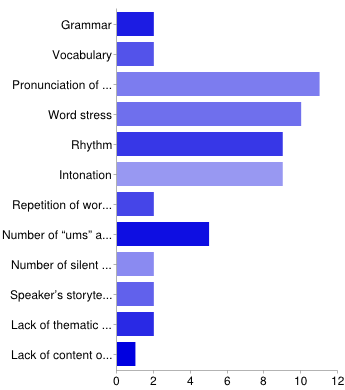
\includegraphics[width=2.3126in,height=2.6146in,width=\textwidth]{delrio-img1.png}
 
\end{styleStandard}


\begin{styleStandard}
Factors from the domain of phonology seemed to contribute the most to listeners’ perception of foreign accent. Both segmental and suprasegmental aspects of speech were selected by most listeners. Pronunciation of individual sounds was selected by 92\% of the listeners, followed by word stress (reported by 83\% of the raters), and rhythm and intonation (75\% each). The next aspect selected by most teachers was “the number of ‘ums’ and ‘uhs’” (42\%), with a considerably lower percentage, however. 
\end{styleStandard}

\begin{styleStandard}
As mentioned above, listeners were also asked to rank the top three aspects that they felt had most influenced their accentedness ratings. As illustrated in Figure 2, the three most selected aspects influencing listeners’ foreign accent ratings were pronunciation of individual sounds, intonation, word stress, and rhythm. Other aspects which were reported by the listeners’ are shown in this figure (e.g. grammar, vocabulary, number of pauses and number of ‘uhms’ and ‘uhs’):
\end{styleStandard}

\begin{styleStandard}
\textit{Figure 2. Aspects affecting listeners’ foreign accent ratings most (\%)}
\end{styleStandard}

\begin{styleStandard}
  [Warning: Image ignored] % Unhandled or unsupported graphics:
%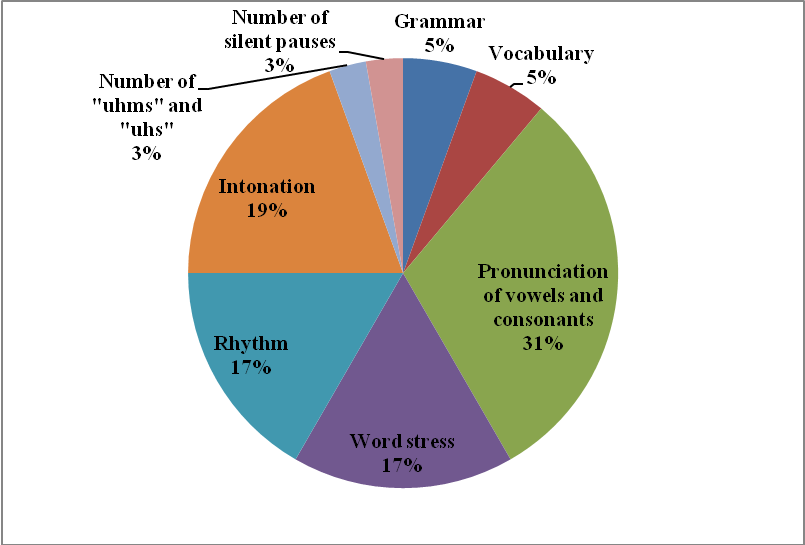
\includegraphics[width=3.3437in,height=2.7811in,width=\textwidth]{delrio-img2.png}
 
\end{styleStandard}


\begin{listWWNumxxiileveli}
\item 
\begin{stylelsSectioniii}
Aspects influencing listeners’ comprehensibility ratings
\end{stylelsSectioniii}

\end{listWWNumxxiileveli}
\begin{styleStandard}
As regards the second part of sub-question two, that is, the analysis of the aspects influencing listeners’ comprehensibility scores, listeners were given a list of 12 aspects and were asked to choose those which had most affected their comprehensibility ratings. The list was identical to the one used for foreign accent and included: grammar, vocabulary, pronunciation, word stress, rhythm, intonation, repetition of words, number of filled pauses with ‘ums’ and similar items, number of silent pauses, speakers’ story telling abilities, lack of thematic content, and lack of content organization. A summary of the results is presented in Figure 3.
\end{styleStandard}

\begin{styleStandard}
\textit{Figure 3. Aspects affecting comprehensibility ratings}
\end{styleStandard}

\begin{styleStandard}
  [Warning: Image ignored] % Unhandled or unsupported graphics:
%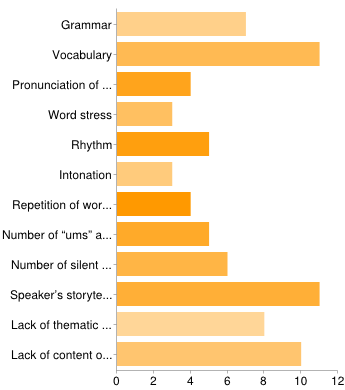
\includegraphics[width=2.2917in,height=2.5937in,width=\textwidth]{delrio-img3.png}
 
\end{styleStandard}


\begin{styleStandard}
Unlike accent, comprehensibility was mostly associated with vocabulary and discourse (storytelling and content organization). More than 90\% of the listeners selected ‘vocabulary’ and ‘speaker’s storytelling ability’, and 83\% bore in mind ‘content organization’ when assigning comprehensibility scores. Lack of thematic content was important for 67\% of the listeners, and grammar influenced the ratings of 60\% of the listeners.
\end{styleStandard}

\begin{styleStandard}
Seventy-five percent of these comments referred to vocabulary. Two listeners pointed out the use of L1 vocabulary as interfering with comprehensibility. The lack of vocabulary was stressed by one of the raters especially. Interestingly, one of the listeners highlighted that speaker’s attitude had also affected her comprehensibility ratings. 
\end{styleStandard}

\begin{styleStandard}
Listeners were also asked to rank the top three aspects that they felt had most influenced their comprehensibility ratings. The three most cited aspects were vocabulary, lack of content organization and speakers’ storytelling ability (followed by grammar and pronunciation of individual sounds). Figure 4 illustrates the results.
\end{styleStandard}

\begin{styleStandard}
\textit{Figure 4. Aspects affecting listeners’’ comprehensibility ratings most (\%)}
\end{styleStandard}

\begin{styleStandard}
  [Warning: Image ignored] % Unhandled or unsupported graphics:
%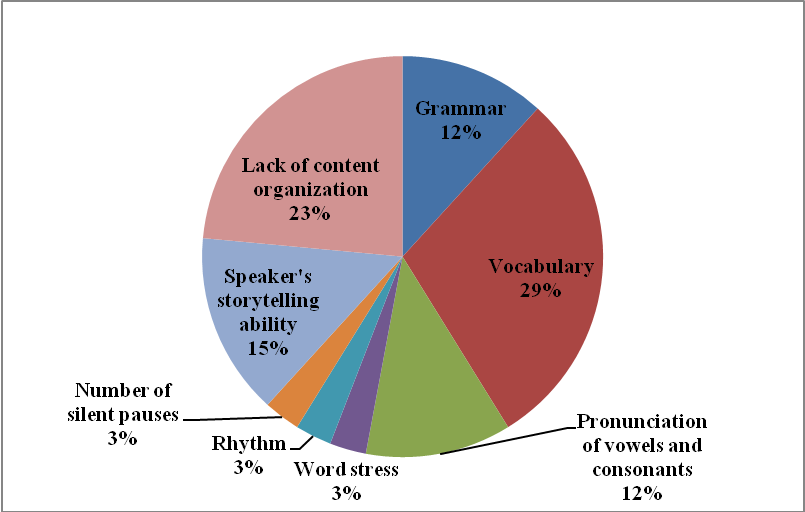
\includegraphics[width=3.802in,height=2.6252in,width=\textwidth]{delrio-img4.png}
 
\end{styleStandard}


\begin{styleStandard}
In order to delve into the comprehensibility construct, we asked listeners to type in their comments immediately after rating the comprehensibility of 20 speech samples scattered throughout the rating experiment. \ We obtained 688 comments about comprehensibility from the text entry boxes which were filled in by the listeners during the rating experiment. The listeners’ descriptive comments were first classified as \textit{indicating a postive or negative remark on the comprehensibility of the sample} . \ There were 426 negative comments and 262 positive comments. Then the comments were thematically coded, and re-coded to eliminate overlapping ones (e.g. ‘L1 word’, ‘invented word’ and ‘wrong word’ were combined under a ‘vocabulary’ category). 
\end{styleStandard}

\begin{styleStandard}
We found that some listeners were more specific than others regarding their comments. Whereas some listeners made general comments about comprehensibility such as “grammar errors,” other listeners specified in their reports the type of grammar errors they found in the participants’ speech (e.g. “no subject,” “wrong verb tense,” etc.). Table 2 shows all the categories obtained from the listeners’ comments indicating whether they were considered as negative (N), or positive (P) evaluations, or both (B). The initial number of comments is provided together with the final number of comments obtained, once double references to the same category made by the same listener were identified (number of comments deleted are indicated in brackets). The percentage of each category over the total number of final comments is indicated in the \% column:
\end{styleStandard}

\begin{styleStandard}
\textit{Table 2. Frequency of coded categories for comprehensibility from teacher reports (initial raw number, final raw number, and \%)}
\end{styleStandard}

\begin{center}
\tablehead{}
\begin{supertabular}{m{1.8893598in}m{1.1261599in}m{0.70875984in}m{0.90665984in}m{0.45315984in}}
\hline
\bfseries Category &
\bfseries Considered as negative, positive or both &
\bfseries Initial number of comments &
\bfseries Final number of comments after recoding &
\bfseries \%\\\hline
\mdseries Ambiguous\footnotemark{} &
\mdseries B &
\mdseries 10 &
\mdseries 10 &
\mdseries 1.67\\
\mdseries Attitude &
\mdseries B &
\mdseries 19 \ (-3) &
\mdseries 16 &
\mdseries 2.68\\
\mdseries Listener’s teaching profile &
\mdseries P &
\mdseries 2 &
\mdseries 2 &
\mdseries 0.33\\
\mdseries Communicative strategies &
\mdseries B &
\mdseries 10 &
\mdseries 10 &
\mdseries 1.67\\
\mdseries Content &
\mdseries B &
\mdseries 37 \ (-1) &
\mdseries 36 &
\mdseries 6.04\\
\mdseries Discourse &
\mdseries B &
\mdseries 61 \ (-12) &
\mdseries 49 &
\mdseries 8.22\\
\mdseries English proficiency &
\mdseries N &
\mdseries 1 &
\mdseries 1 &
\mdseries 0.16\\
\mdseries Familiarity with the story &
\mdseries P &
\mdseries 4 &
\mdseries 4 &
\mdseries 0.67\\
\mdseries \textbf{Fluency} &
\mdseries \textbf{B} &
\mdseries 97 \ (-11) &
\mdseries 86 &
\mdseries \textbf{14.42}\\
\mdseries \textbf{Grammar} &
\mdseries \textbf{B} &
\mdseries 99 \ (-12) &
\mdseries 87 &
\mdseries \textbf{14.59}\\
\mdseries L1 familiarity &
\mdseries B &
\mdseries 16 \ (-2) &
\mdseries 14 &
\mdseries 2.34\\
\mdseries L1 influence (general comment) &
\mdseries N &
\mdseries 3 &
\mdseries 3 &
\mdseries 0.50\\
\mdseries Listener’s attitude &
\mdseries P &
\mdseries 4 &
\mdseries 4 &
\mdseries 0.67\\
\mdseries Low voice &
\mdseries N &
\mdseries 3 &
\mdseries 3 &
\mdseries 0.50\\
\mdseries \textbf{Pronunciation} &
\mdseries \textbf{B} &
\mdseries 194 \ \ (-39) &
\mdseries 155 &
\mdseries \textbf{26}\\
\mdseries Self-correction &
\mdseries P &
\mdseries 4 &
\mdseries 4 &
\mdseries 0.67\\
\mdseries Style &
\mdseries B &
\mdseries 3 \ \ \ (-1) &
\mdseries 2 &
\mdseries 0.33\\
\mdseries \textbf{Vocabulary} &
\mdseries \textbf{B} &
\mdseries 121 \ \ (-11) &
\mdseries 110 &
\mdseries \textbf{18.45}\\\hline
\end{supertabular}
\end{center}
\footnotetext{ There were a number of comments which were categorized as ‘Ambiguous’. They were included in this category when it was not clear what the listeners were considering. For instance, for comments such as “I can{\textquotesingle}t understand some words{\textquotedbl}, it was not clear whether there was a pronunciation problem on the part of the speaker or if the speaker had invented a word which the listener could not understand (vocabulary). Given that we were not sure \ whether this was a comment referred to pronunciation or vocabulary, we assigned it to the ‘Ambiguous’ category.\par \textsuperscript{2 }The data collection procedure comprised 3 academic years since data was collected from two consecutive cohorts of students at the same home institution.\par \textsuperscript{3 }Data from NSs was collected by researchers at the\textit{ Universitat de les Illes Balears} participating in the SALA and COLE research projects, coordinated by \textit{Universitat Pompeu Fabra} (Barcelona, Spain). \par }
\begin{styleStandard}
As can be observed, 26\% of the comments referred to pronunciation (including segmental and supra-segmental aspects). Vocabulary was the second most frequent aspect considered by listeners in their comments (18.45\%), followed by grammar (14.59\%) and fluency (14.42\%). \ 
\end{styleStandard}

\begin{styleStandard}
Further analyses explored whether the above-mentioned aspects were also taken into account to a similar extent in negative and positive comprehensibility ratings. Therefore, we examined the 426 negative comments and the 262 positive ones separately.
\end{styleStandard}

\begin{styleStandard}
As for the comments identifying negative evaluations of comprehensibility, pronunciation, vocabulary and grammar were reported as the categories that most frequently affected listeners’ scoring decisions. Twenty-six percent of the comments referred to segmental and supra-segmental aspects of participants’ speech, 22.71\% dealt with vocabulary items, and 19.11\% with grammar. Fluency was mentioned in almost 15\% of the comments. Table 3 shows the results of this analysis.
\end{styleStandard}

\begin{styleStandard}
\textit{Table 3. Frequency of coded categories for negative comments on comprehensibility from teacher reports (initial raw number, final raw number, and \%).}
\end{styleStandard}

\begin{center}
\tablehead{}
\begin{supertabular}{m{1.8900598in}m{0.70875984in}m{0.6754598in}m{0.6434598in}}
\hline
\bfseries Category &
\bfseries Initial number of comments &
\bfseries Final number of comments &
\bfseries \%\\\hline
\mdseries Ambiguous &
\mdseries 7 &
\mdseries 7 &
\mdseries 1.93\\
\mdseries Attitude &
\mdseries 10 &
\mdseries 8 &
\mdseries 2.21\\
\mdseries Communicative strategies &
\mdseries 1 &
\mdseries 1 &
\mdseries 0.27\\
\mdseries Content &
\mdseries 19 &
\mdseries 19 &
\mdseries 5.26\\
\mdseries Discourse &
\mdseries 20 &
\mdseries 19 &
\mdseries 5.26\\
\mdseries English proficiency &
\mdseries 1 &
\mdseries 1 &
\mdseries 0.27\\
\mdseries \textbf{Fluency} &
\mdseries 62 &
\mdseries 53 &
\mdseries \textbf{14.68}\\
\mdseries \textbf{Grammar} &
\mdseries 80 &
\mdseries 69 &
\mdseries \textbf{19.11}\\
\mdseries (No) L1 familiarity &
\mdseries 3 &
\mdseries 1 &
\mdseries 0.27\\
\mdseries L1 influence (general comment) &
\mdseries 3 &
\mdseries 3 &
\mdseries 0.83\\
\mdseries Low voice &
\mdseries 1 &
\mdseries 3 &
\mdseries 0.83\\
\mdseries \textbf{Pronunciation} &
\mdseries 126 &
\mdseries 94 &
\mdseries \textbf{26.03}\\
\mdseries Style &
\mdseries 2 &
\mdseries 1 &
\mdseries 0.27\\
\mdseries \textbf{Vocabulary} &
\mdseries 91 &
\mdseries 82 &
\mdseries \textbf{22.71}\\
\mdseries \textbf{Total} &
\mdseries 426 &
\mdseries 361 &
\\\hline
\end{supertabular}
\end{center}
\begin{styleStandard}
To have a better idea of the pronunciation features, we classified the comments according to the aspect of speech they were more specifically referring to. Table 4 shows this classification and the percentage of comments assigned to each pronunciation category.
\end{styleStandard}

\begin{styleStandard}
\textit{Table 4. Pronunciation aspects reported by listeners as negatively influencing their comprehensibility ratings of participants’ speech}
\end{styleStandard}

\begin{center}
\tablehead{}
\begin{supertabular}{m{2.6768599in}m{0.6101598in}}
\hline
\bfseries Pronunciation aspect &
\bfseries \%\\\hline
\mdseries Pronunciation of individual sounds and words &
\mdseries 55.55\\
\mdseries Foreign accent &
\mdseries 17.46\\
\mdseries Intonation &
\mdseries 11.11\\
\mdseries Rhythm &
\mdseries 3.96\\
\mdseries Stress &
\mdseries 2.3\\
\mdseries Native-like pronunciation &
\mdseries 4\\
\mdseries Other\footnotemark{} &
\mdseries 5.55\\\hline
\end{supertabular}
\end{center}
\footnotetext{ Comments regarding pronunciation in general and speech clarity were categorized under the ‘Other’ category. }
\begin{styleStandard}
Half of the comments regarding pronunciation problems referred to the pronunciation of individual sounds or words. It is worth remarking that specific reference was made to foreign-accented speech as an aspect affecting comprehensibility (17\% of the comments referred to foreign accent). However, ‘L1 interference’ was mentioned when considering other pronunciation factors such as pronunciation of individual sounds or words, and intonation. Comments such as “Spanish intonation,” “L1 influence on pronunciation” and “typical pronunciation mistake (from their L1)” were collected.
\end{styleStandard}

\begin{styleStandard}
Having a native-like pronunciation was regarded as hindering comprehensibility to some extent by some of the listeners when rating native participants’ speech. Comments such as those in (3) were collected from listeners’ evaluations: 
\end{styleStandard}

\setcounter{listWWNumxleveli}{0}
\begin{listWWNumxleveli}
\item 
\begin{stylelsEnumerated}
ELME: “after listening to so many recordings with the same type of syllable-timed speech, it was hard to readjust my ear to connected speech”~
\end{stylelsEnumerated}

\end{listWWNumxleveli}
\begin{styleStandard}
As regards the comments referring to aspects positively affecting comprehensibility ratings, pronunciation was also considered the most influential aspect. As shown in Table 5, fluency, discourse and vocabulary were aspects reported in more than 10\% of the comments.
\end{styleStandard}

\begin{styleStandard}
\textit{Table 5. Frequency of coded categories for positive comments on comprehensibility from teacher reports (initial raw number, final raw number, and \%)}
\end{styleStandard}

\begin{center}
\tablehead{}
\begin{supertabular}{m{1.8900598in}m{0.70875984in}m{0.6754598in}m{0.6434598in}}
\hline
\bfseries Category &
\bfseries Initial number of comments &
\bfseries Final number of comments &
\bfseries \%\\\hline
\mdseries Ambiguous &
\mdseries 3 &
\mdseries 3 &
\mdseries 1.23\\
\mdseries Attitude &
\mdseries 9 &
\mdseries 8 &
\mdseries 3.29\\
\mdseries Being a teacher &
\mdseries 2 &
\mdseries 2 &
\mdseries 0.82\\
\mdseries Communicative strategies &
\mdseries 9 &
\mdseries 9 &
\mdseries 3.70\\
\mdseries Content &
\mdseries 18 &
\mdseries 17 &
\mdseries 7\\
\mdseries \textbf{Discourse} &
\mdseries 41 &
\mdseries 31 &
\mdseries \textbf{12.75}\\
\mdseries Familiarity with the story &
\mdseries 4 &
\mdseries 4 &
\mdseries 1.64\\
\mdseries \textbf{Fluency} &
\mdseries 35 &
\mdseries 34 &
\mdseries \textbf{14}\\
\mdseries Grammar &
\mdseries 19 &
\mdseries 19 &
\mdseries 7.81\\
\mdseries L1 familiarity &
\mdseries 15 &
\mdseries 13 &
\mdseries 5.34\\
\mdseries Listener’s attitude &
\mdseries 4 &
\mdseries 4 &
\mdseries 1.64\\
\mdseries \textbf{Pronunciation} &
\mdseries 68 &
\mdseries 63 &
\mdseries \textbf{26.33}\\
\mdseries Self-correction\ \  &
\mdseries 4 &
\mdseries 4 &
\mdseries 1.64\\
\mdseries Style &
\mdseries 1 &
\mdseries 1 &
\mdseries 0.41\\
\mdseries \textbf{Vocabulary} &
\mdseries 30 &
\mdseries 30 &
\mdseries \textbf{12.34}\\
\mdseries Total  &
\mdseries 262 &
\mdseries 242 &
\\\hline
\end{supertabular}
\end{center}
\begin{styleStandard}
As with the pronunciation comments identifying negative aspects of participants’ speech comprehensibility, we analyzed listeners’ reports on positive evaluations in further depth and found that listeners did not identify any particular aspects of pronunciation as positively affecting their comprehensibility ratings, but rather they referred to pronunciation in general. About 40\% of the comments were similar to the following ones: “quite good pronunciation that facilitates comprehensibility,” “pronunciation is OK,” and “pronunciation is not that bad”. Having a native-like pronunciation or imitating native-like pronunciation was the second most frequently cited aspect (22\% of the comments). Moreover, general comments on accent were reported in 15\% of the listeners’ comments (e.g. “good accent”). Table 6 shows the percentage of comments assigned to each pronunciation aspect reported by the listeners as positively affecting their comprehensibility ratings.
\end{styleStandard}

\begin{styleStandard}
\textit{Table 6. Pronunciation aspects reported by listeners as positively influencing their comprehensibility ratings of participants’ speech}
\end{styleStandard}

\begin{center}
\tablehead{}
\begin{supertabular}{m{2.6768599in}m{0.6101598in}}
\hline
\bfseries Pronunciation aspect &
\bfseries \%\\\hline
\mdseries Pronunciation of individual sounds and words &
\mdseries 2.94\\
\mdseries Accent (general comment) &
\mdseries 14.7\\
\mdseries Intonation &
\mdseries 10.29\\
\mdseries Rhythm &
\mdseries 7.35\\
\mdseries Pronunciation (general positive comment) &
\mdseries 41.17\\
\mdseries Native or imitating native-like pronunciation &
\mdseries 22.05\\
\mdseries Being familiar with L1 accent &
\mdseries 1.47 \\\hline
\end{supertabular}
\end{center}
\begin{styleStandard}
While language aspects such as pronunciation, vocabulary, grammar or fluency were most frequently reported by listeners as affecting comprehensibility, other aspects were mentioned which will be discussed in more detail in the following section. Reference to a NS model or the importance of native-like speech, L1 familiarity and the speaker’s and listener’s attitude were points made by the listeners which will also receive special attention in the next pages so as to provide further answers and comments in the context of English pronunciation teaching today.
\end{styleStandard}

\setcounter{listWWNumxxiileveli}{0}
\begin{listWWNumxxiileveli}
\item 
\begin{stylelsSectioni}
Discussion
\end{stylelsSectioni}

\end{listWWNumxxiileveli}
\begin{styleStandard}
The main research question in this study enquired as to whether or not and to what\textbf{ }extent foreign accent and comprehensibility are related speech dimensions when judged by non-native listeners, in the case of a group of EFL learners experiencing a SA period, and another group experiencing a FI period at home, and what aspects affected their decisions. 
\end{styleStandard}

\begin{styleStandard}
Our results have revealed significant large positive correlations between the two speech dimensions at the two testing times, that is before and after both FI and SA, for both groups of participants, indicating that the more native-like the accent, the greater the comprehensibility, and vice-versa. These results contrast with those reported in previous studies positing that heavily accented speech can often be perfectly intelligible, which, in contrast had mostly naïve (that is, non-language professionals) NSs as listeners (Munro \& Derwing 1995; 1999; Derwing \& Munro 1997; Gallardo del Puerto et al. 2007; Hayes-Harb \& Watzinger-Tharp 2012). One possible interpretation of these findings is that the sample is rather homogeneous, both in the speakers and in the listeners: The learners who provided the speech samples have been attending the same FI class during their former education prior to data collection, and the listeners are non-native EFL teachers, who train their students to try and achieve native-like standards. For them accent may actually indeed interfere with comprehension. Another interesting result was the fact that none of the participants were assigned a high foreign accent rating and a low comprehensibility score. In other words, participants who were assigned high comprehensibility scores were also given good ratings in foreign accent.
\end{styleStandard}

\begin{styleStandard}
Given these three results – that is, (1) positive correlations between foreign accent and comprehensibility (the better the ratings in foreign accent, the higher the ratings in comprehensibility), (2) learners’ approximation to native-like accent always associated with good comprehensibility ratings, and (3) a contrast with the extant literature regarding the link established by listeners between accent and comprehensibility – our sub-question 2, which taps into the aspects which influenced listeners’ foreign accent and comprehensibility ratings, gained more relevance. Qualitative analyses were thus conducted of listeners’ comments gathered from the questionnaires they completed after finishing the rating task, and from 20 reports which were typed in at the same time that they provided their ratings during the rating task. 
\end{styleStandard}

\begin{styleStandard}
Concerning the aspects affecting foreign accent ratings, factors from the domain of phonology were selected from the list by most listeners (see Figure 1). Pronunciation of vowels/consonants, word stress, rhythm and intonation were reported in this order as mainly affecting their foreign accent assessment. This finding was confirmed when listeners were asked which three aspects had influenced their foreign accent ratings most (see Figure 2). Pronunciation of vowels/consonants, intonation, word stress and rhythm were considered in this order. In fact, these phonological dimensions altogether represented 84\% of the factors selected by the listeners as mostly influencing their foreign accent ratings. These results confirmed the findings in Trofimovich \& Isaacs (2012) indicating that accent was mainly associated with aspects of phonology (e.g. rhythm, segmental accuracy, and syllable structure).
\end{styleStandard}

\begin{styleStandard}
On the other hand, comprehensibility was mostly related to vocabulary and discourse aspects, such as storytelling and content organization (see Figure 3). Lack of thematic content and grammar were also selected by more than half of the listeners. When asked to identify the three most influential aspects on their comprehensibility ratings (Figure 4), vocabulary (29\%), lack of content organization (23\%) and speaker’s storytelling ability (15\%) were reported in this order, followed by grammar (12\%) and pronunciation of individual sounds (12\%). 
\end{styleStandard}

\begin{styleStandard}
If we now consider the last part of sub-question 2, which tapped into whether listeners’ foreign accent and comprehensibility ratings were based on similar aspects of the learners’ oral productions, it is worth noting that even though none of the phonological factors were as important individually for the comprehensibility ratings as in the case of the foreign accent ratings, pronunciation of vowels and consonants represented 12\% of the comments, word stress 3\% and rhythm 3\%. All these phonological factors taken together represented 18\% of the comments related to comprehensibility ratings, a higher percentage than, for instance, speaker’s storytelling ability, which was ranked third in the list presented above of the most influential factors affecting listeners’ assessment of comprehensibility. 
\end{styleStandard}

\begin{styleStandard}
These results are in line with Trofimovich \& Isaacs’ (2012) findings, which indicated that comprehensibility was mainly linked to grammatical accuracy and lexical richness. As seen in the literature review, Trofimovich \& Isaacs (2012) identified five speech aspects which differentiated between L2 learners at different comprehensibility levels: lexical richness and fluency distinguished between low-level learners, grammatical and discourse-level measures differentiated between high-level learners, and word stress errors discriminated between learners of all levels. Overall results in our study suggest that listeners regarded vocabulary and also discourse aspects (lack of content organization and speaker’s storytelling ability) as the most important factors related to comprehensibility, factors which were also indicated in Trofimovich \& Isaacs’ (2012) research. However, findings in our research do not support Trofimovich \& Isaacs’ conclusion pointing out that “four categories uniquely distinguished accent from comprehensibility, with all categories specific to the dimension of phonology (i.e., vowels and consonants, syllables, sounding native-like, and rhythm)” (p. 912). \ \ As we have seen, pronunciation aspects (e.g. pronunciation of individual sounds) were also taken into account by the listeners in our study when assessing comprehensibility. As suggested above, the differences in listeners’ profiles in both studies, non-native language specialists in the current study versus naïve NSs in prior works, might be the reason for this discrepancy. 
\end{styleStandard}

\begin{styleStandard}
It is worth mentioning other aspects (different from the ones provided in the list) which some of the listeners reported as having influenced their comprehensibility ratings. Almost all comments referred to vocabulary, and some of them stressed the use of L1 items as hampering comprehensibility, as in (4). 
\end{styleStandard}

\setcounter{listWWNumxleveli}{0}
\begin{listWWNumxleveli}
\item 
\begin{stylelsEnumerated}
INCA: “Use of Spanish words maybe”\footnote{ L1 lexical interference was confirmed to negatively affect INCA’s comprehensibility ratings, as she reported other comments throughout the perception task such as, “use of words translated from Spanish (“senior”, from Spanish word “señor” -meaning “man”). \par }. 
\end{stylelsEnumerated}

\end{listWWNumxleveli}
\begin{stylelsEnumerated}
MOLO: “The use of L1 words in some cases which shows the lack of ability of the student to make the message be understood”
\end{stylelsEnumerated}


\begin{styleStandard}
The fact that these listeners considered the use and transfer of L1 words as negatively affecting comprehensibility does not necessarily contradict findings in previous studies suggesting the speech comprehensibility benefit for NNSs and non-native listeners sharing the same L1 background (Hayes-Harb et al. 2008; Gallardo del Puerto et al. 2009), mentioned previously. However, the analysis of all the comments gathered from listeners, including those in (5), showed that L1 lexical interference was not positively considered in many instances.
\end{styleStandard}

\begin{listWWNumxleveli}
\item 
\begin{stylelsEnumerated}
COGA: “The use of Spanish words makes it confusing”
\end{stylelsEnumerated}

\end{listWWNumxleveli}
\begin{stylelsEnumerated}
INCA: “usa vocabulario {\textquotedbl}traducido{\textquotedbl} de la lengua materna” (‘\textit{He “translates” words from his L1}’). 
\end{stylelsEnumerated}


\begin{stylelsEnumerated}
MAGU: “Clara influencia de la lengua materna. Adapta claramente vocabulario al inglés. Es dificil de comprender por el vocabulario” (‘\textit{Clear influence of his L1. }\textit{He adapts lexical items from his L1. It’s difficult to understand because of the vocabulary}’).
\end{stylelsEnumerated}


\begin{styleStandard}
So far, our results partly support those reported by recent research indicating that foreign accent and comprehensibility are linked to different language aspects. On the one hand, we can conclude that aspects of phonology affected foreign accent ratings more than aspects related to other domains such as grammar or vocabulary. On the other hand, although results confirmed that vocabulary and discourse factors, as well as grammar, were the main contributors to variation in comprehensibility ratings, reports from the listeners in our study suggested that factors related to pronunciation also had some influence on their assessment of comprehensibility, when considering the data from the two learning contexts together. 
\end{styleStandard}

\begin{styleStandard}
The listeners were also asked to type in the aspects of speech which they were taking into account when providing their comprehensibility ratings. Responses for 20 of the speech samples were analyzed. The analyses of these comments helped us to elucidate whether pronunciation was actually involved (or not) in listeners{\textquotesingle} comprehensibility ratings. 
\end{styleStandard}

\begin{styleStandard}
When analyzing all the comments provided by the listeners we found that 26\% of the comments regarding their comprehensibility ratings considered aspects of pronunciation, 18.45\% of the comments referred to vocabulary, 14.59\% to grammar, and 14.42\% to fluency. Therefore, a new distribution of the aspects affecting this speech dimension was obtained (compared to the 12-item classification from the final questionnaires presented above). Vocabulary was considered a key aspect for comprehensibility in many of the comments, but pronunciation was even more frequently highlighted. 
\end{styleStandard}

\begin{styleStandard}
The comments from the reports were classified as affecting negatively or positively the listeners’ ratings. With regard to the aspects hindering comprehensibility, 26\% of the comments were related to pronunciation, 22.71\% associated with vocabulary, and 19\% linked to grammar. Pronunciation was also regarded as the variable enhancing comprehensibility most. Twenty-six percent of the comments providing reasons for good comprehensibility had to do with pronunciation, 14\% were related to fluency, 12.75\% to discourse, and 12.34\% were associated with vocabulary. 
\end{styleStandard}

\begin{styleStandard}
Therefore, according to these analyses, comprehensibility was related to pronunciation to a considerable degree. In order to gain a better understanding of the pronunciation aspects promoting (or hampering) comprehensibility, we classified the comments according to the pronunciation features which the listeners were particularly referring to. The top three pronunciation features which were mentioned in negative evaluations of comprehensibility were pronunciation of individual sounds and words (55.5\%), foreign accent (17.42\%), and intonation (11.1\%). As for the pronunciation aspects which were identified in positive comments on comprehensibility, listeners cited pronunciation in general (41.1\%), imitation of native-like pronunciation (22\%), and degree of accentedness (14.7\%), followed by intonation (10.29\%).
\end{styleStandard}

\begin{styleStandard}
Therefore, according to the reports on comprehensibility provided by the listeners while carrying out the perception task, pronunciation was found to be the most relevant aspect in their assessment of comprehensibility of L2 learners{\textquotesingle} speech. \ The fact that pronunciation was not ranked within the top three aspects affecting comprehensibility in the data obtained from the questionnaires may potentially be explained in two ways. First, since we presented the questions about the factors influencing foreign accent and comprehensibility ratings in the same questionnaire, we could have implicitly motivated the distinction between the two constructs. Second, as already remarked, while it is true that specific pronunciation features (e.g. pronunciation of individual sounds, intonation, stress, etc.) did not greatly affect comprehensibility when considered separately, pronunciation aspects taken as a whole did have a considerable impact on the listeners’ comments. On the other hand, we may consider the comments made by the listeners during the rating experiment as more reliable and ecologically valid than the comments collected at the end of the experiment, as the former were reported when listeners were actually rating the speech samples for comprehensibility. 
\end{styleStandard}

\begin{styleStandard}
According to these data, non-native listeners in our study took into account pronunciation aspects when assessing L2 learners’ comprehensibility of English, both after FI and SA. First, strong positive correlations between foreign accent and comprehensibility were found for data from both contexts, in spite of the fact that these contexts might have affected learners differently. Second, listeners in our study did pay attention to aspects related to accent or native-like pronunciation when providing their comprehensibility ratings with data from both contexts, in contrast with previous research involving native listeners of English (Trofimovich \& Isaacs 2012). Against such backdrop, further research is needed to gain a better understanding of the aspects affecting comprehensibility as reported by native and non-native listeners.
\end{styleStandard}

\setcounter{listWWNumxxiileveli}{0}
\begin{listWWNumxxiileveli}
\item 
\begin{stylelsSectioni}
Conclusion
\end{stylelsSectioni}

\end{listWWNumxxiileveli}
\begin{styleStandard}
In this research study we have examined foreign accent and comprehensibility ratings assigned by English non-native instructors, who are frequently responsible for teaching FI EFL courses in the AH context in Spain, so as to determine the relationship between these two speech dimensions, in the case of a group of EFL learners experiencing a SA period, and another group experiencing a FI period at home. Contrary to previous findings (Munro \& Derwing 1999; Derwing \& Munro 2009), a strong correlation has been found between foreign accent and comprehensibility, indicating that those learners with better accent obtained higher comprehensibility ratings, and learners with heavier foreign accent were also perceived as less comprehensible. Furthermore, we have explored the aspects that listeners took into account when assessing foreign accent and comprehensibility. Results showed that the foreign accent dimension was mainly associated with pronunciation aspects, which also affected comprehensibility ratings assigned by the non-native listeners in our research. Confirming previous research (Trofimovich \& Isaacs 2012), aspects such as vocabulary and grammar were taken into account when rating L2 learners’ speech comprehensibility but, contrary to previous findings in studies involving native listeners of English, pronunciation was the aspect that listeners heeded most when assigning comprehensibility scores. 
\end{styleStandard}

\begin{styleStandard}
It remains unclear whether the aspects reported by the group of non-native listeners of our study are specific to our participants, or can be generalized to learners from different L1 backgrounds, or experiencing other learning contexts besides FI and SA, such as, for example, immersion classrooms. In addition, it would be advisable to validate our findings with English native and non-native listeners from other L1 backgrounds and profiles. Likewise, when considering the 12 factors that influence foreign accent and comprehensibility ratings the most, the preponderance of aspects that concern phonetics should guide our analyses in future, paired with a more careful weighting of the factors included in the list. In these respects further research is necessary to throw more light on this area of speech production abilities, in the case of EFL adolescent learners. 
\end{styleStandard}

\begin{styleStandard}
One of the findings in our study is the difference between ratings given by listeners who are language specialists, sharing their L1 with the learners’ whose samples they are rating, as opposed to naïve NSs. More research seems necessary in order to add further evidence to allow us to disentangle those two variables which now seem to be conflated and tackle the issue of listerners’ profile under this new light. Finally, although it is widely accepted that the objective of L2 pronunciation teaching should be to help L2 learners be understandable for their interlocutors, classroom teachers have received little guidance on the pronunciation features on which they should focus during lessons (Derwing \& Munro 2009). Nonetheless, teaching pronunciation should be even more important in the case of EFL learners facing a period of residence abroad, during which issues of comprehensibility and accentedness may impinge on the efficacy learners display in establishing interaction with target language speakers, and being seen as possible interlocutors in communicative encounters. The fact that pronunciation tends to suffer from neglect may not be due to teachers’ lack of interest in the subject but rather to a feeling of doubt as to how to teach it. Another factor affecting the teaching of pronunciation these days may be the popular idea that one learns it best while being in the target language country, hence during SA programmes. Even if this may be partially true, current research on SA emphasizes the need for preparation before departure as it has been observed to correlate very highly with progress made while abroad (Paige et al. 2002). Lack of knowledge of phonetics and lack of formal preparation to teach pronunciation are two of the most cited problems, which have been corroborated in our research. The urgent need for specific pronunciation training for teachers in Spain has been called for frequently (Levey 1999; 2001; Donovan 2001; Pavón 2001; Pavón \& Rosado 2003). In this regard, it is worth highlighting the willingness reported by listeners to benefit from pronunciation training programs and participation in studies like this one, which have provided them with food for thought. 
\end{styleStandard}

\begin{styleStandard}
In sum, the current study has sought to make several contributions to the field of speech production studies. Firstly, it hopes to contribute to the field by offering an analysis of \ the L2 speech dimensions of accentedness and comprehensibility in the case of SA EFL learners. By having done so we have increased the number of studies examining these dimensions in the speech production of adolescent EFL learners, who experience the two learning environments mentioned above, FI and SA, a clearly underresearched population. Secondly, we sought to contribute to bridging the gap between research and language teaching practice in the face of the number of learning contexts which learners can experience, such as FI and SA, to name but two. Although further studies need to be conducted in order to confirm and generalize our findings, ours is a modest but ecologically valid contribution to empirical-based research aiming at exploring what really happens with regard to the assessment of pronunciation.
\end{styleStandard}

\begin{stylelsSectioni}
References
\end{stylelsSectioni}


\begin{styleStandard}
Dalton, Christiane \& Seidlhofer, Barbara (1994). Pronunciation. Oxford: Oxford University Press.
\end{styleStandard}


\begin{styleStandard}
Derwing, Tracey M. (2008). Curriculum issues in teaching pronunciation to second language learners. In Hansen Edwards, Jette G. \& Zampini, Mary L. (Eds.), Phonology and Second Language Acquisition (pp. 347-369). Amsterdam: John Benjamins Publishing Company.
\end{styleStandard}


\begin{styleStandard}
Derwing, Tracey M. \& Munro, Murray J. (1997). Accent, intelligibility, and comprehensibility: Evidence from four L1s. \textit{Studies in Second Language Acquisition, }19, 1-16. 
\end{styleStandard}


\begin{styleStandard}
Derwing, Tracey M. \& Munro, Murray J. (2009). Putting accent in its place: Rethinking obstacles to communication. \textit{Language Teaching}, 42(4), 476 – 490.
\end{styleStandard}


\begin{styleStandard}
Derwing, Tracey M. \& Munro, Murray J. (2011). Second language accent and pronunciation teaching: a research-based approach. \textit{TESOL Quarterly}, 39 (3), 379 – 397.
\end{styleStandard}


\begin{styleStandard}
Derwing, Tracey M. \& Munro, Murray J. (2013). The development of L2 oral language skills in two L1 groups: a 7-year study. \textit{Language Learning}, 63 (2), 163-185.
\end{styleStandard}


\begin{styleStandard}
Derwing, Tracey M., Munro, Murray J., \& Wiebe, Grace (1998). Evidence in favor of a broad framework for pronunciation instruction. \textit{Language Learning}, 48, 393-410. 
\end{styleStandard}


\begin{styleStandard}
Donovan, Patrick J. (2001). Making Pronunciation a Priority for EFL Teachers and Learners. In Levey, David T., Losey León, María Araceli \& González macías, Miguel Ángel (Eds.). \textit{English Language Teaching Changing Perspectives in Context} (pp.245-249). Cádiz: Universidad de Cádiz (Servicio de Publicaciones).
\end{styleStandard}


\begin{styleStandard}
Dörnyei, Zoltán (2007). \textit{Research methods in applied linguistics}. Oxford: Oxford University Press. 
\end{styleStandard}


\begin{styleStandard}
Fisher, Linda \& Evans, Michael (2000). The school exchange visit: effects on attitudes and proficiency in language learning. \textit{Language Learning Journal}, 22, 11-16. 
\end{styleStandard}


\begin{styleStandard}
Gallardo del Puerto, Francisco, Gómez Lacabex, Esther \& García Lecumberri, María Luisa (2009). Testing the effectiveness of Content and Language Integrated Learning in foreign language contexts: The assessment of English pronunciation. In Ruiz de Zarobe, Y., \& Jiménez Catalán, R. M. (Eds.), Content and Language Integrated Learning. Evidence from research in Europe (pp. 63-80). Clevedon: Multilingual Matters.
\end{styleStandard}


\begin{styleStandard}
García Lecumberri, María Luisa \& Gallardo del Puerto, Francisco (2003). English FL sounds in school learners of different ages. In García-Mayo, María del Pilar, García-Lecumberri, María Luisa (eds.), \textit{Age and the Acquisition of English as a Foreign Language} (pp. 115-135). Clevedon, England: Multilingual Matters.
\end{styleStandard}


\begin{styleStandard}
Gass, Susan \& Varonis, Evangeline (1984). The effect of familiarity on the comprehensibility of nonnative speech. \textit{Language Learning}, 34, 65–89.
\end{styleStandard}


\begin{styleStandard}
Gimson, Alfred Charles (1994) Gimson’s pronunciation of English. Revision by Alan Cruttenden. London: Edward Arnold.
\end{styleStandard}


\begin{styleStandard}
Hayes-Harb, Rachel \& Watzinger{}-Tharp, Johanna (2012) Accent, intelligibility, and the role of the listener: perceptions of English-accented German by native German speakers. \textit{Foreign Language Annals}, 45, 260-282.
\end{styleStandard}


\begin{styleStandard}
Isaacs, Talia (2010). \textit{Issues and arguments in the measurement of second language pronunciation}. PhD Thesis, McGill University, Montreal. 
\end{styleStandard}


\begin{styleStandard}
Isaacs, Talia \& Trofimovich, Pavel (2012). “Deconstructing” comprehensibility: Identifying the linguistic influences on listeners’ L2 comprehensibility ratings. \textit{Studies in Second Language Acquisition}, 34, 475-505.
\end{styleStandard}


\begin{styleStandard}
Jenkins, Jennifer (2000)\textit{. The phonology of English as an International language.} Oxford: Oxford University Press. 
\end{styleStandard}


\begin{styleStandard}
Kenworthy, Joanne (1987). Teaching English pronunciation. London: Longman.
\end{styleStandard}


\begin{styleStandard}
Kennedy, Sara \& Trofimovich, Pavel (2008). Intelligibility, comprehensibility, and accentedness of L2 speech: The role of listener experience and semantic context. \textit{Canadian Modern Language Review}\textit{64.}459–489.
\end{styleStandard}


\begin{styleStandard}
Llanes, Àngels (2012). The short and long-term effect of a short study abroad experience. \textit{System},\textit{ 40}, 179-190.
\end{styleStandard}


\begin{styleStandard}
Llanes, Àngels, \& Muñoz, Carmen (2012). Age effects in a study abroad context: Children and adults studying abroad and at home. \textit{Language Learning},\textit{ 64}(1)\textit{, }1-28.
\end{styleStandard}


\begin{styleStandard}
Levey, David Trevor (1999). Half Truths and White Lies: A Practical Pronunciation Guide for Spanish Speakers. In Harris, Tony \& Sanz Sainz, Inmaculada (Eds.) ELT: \textit{Through the Looking Glass }(pp. 215-226)\textit{. }Granada: Greta.
\end{styleStandard}


\begin{styleStandard}
Levey, David Trevor (2001). Stressing Intonation. In Harris, Tony, Roldan Miranda, María Inmaculada, Sanz Sainz, Inmaculada, \&. Torreblanco Sojo, Montserrat (Eds.) \textit{ELT2000}: \textit{Thinking Back, Looking Forward }(pp. 35-45)\textit{. }Granada: Greta.
\end{styleStandard}


\begin{styleStandard}
Levis, John M. (2005). Changing contexts and shifting paradigms in pronunciation teaching. \textit{TESOL Quarterly}, 39, 369-377.
\end{styleStandard}


\begin{styleStandard}
Levis, John M. (2006). Pronunciation and the assessment of spoken language. In Hughes, Rebecca (Ed.), \textit{Spoken English, TESOL and applied linguistics}: \textit{Challenges for theory and practice} (pp. 245 - 270). New York: Palgrave Macmillan. 
\end{styleStandard}


\begin{styleStandard}
Munro, Murray J. (2008). Foreign accent and speech intelligibility. In Hansen Edwards, Jette G., \& Zampini, Mary L. (Eds.), \textit{Phonology and Second Language Acquisition} (pp. 193-218). Amsterdam: John Benjamins Publishing Company.
\end{styleStandard}


\begin{styleStandard}
Munro, Murray J., \& Derwing, Tracey M. (1995). Foreign accent, comprehensibility, and intelligibility in the speech of second language learners. \textit{Language Learning}, 45(1), 73–97.
\end{styleStandard}


\begin{styleStandard}
Munro, Murray J. \& Derwing, Tracey M. (1999). Foreign accent, comprehensibility, and intelligibility in the speech of second language learners. \textit{Language Learning}, 49, 285–310.
\end{styleStandard}


\begin{styleStandard}
Paige, R. Michael, Cohen, Andrew D. \& Shiveley, Rachel L. (2002). Assessing the impact of a strategies-based curriculum on language and culture learning while abroad. \textit{Frontiers: The Interdisciplinary Journal of Study Abroad (v10), }253-276.
\end{styleStandard}


\begin{styleStandard}
Pavón Vázquez, Víctor (2001). El Papel del Profesor en la Enseñanza de la Pronunciación. In Levey, David T., Losey León, María Araceli, \& González macías, Miguel Ángel (Eds.). \textit{English Language Teaching Changing Perspectives in Context} (pp. 289-300). Cádiz: Universidad de Cádiz (Servicio de Publicaciones). 
\end{styleStandard}


\begin{styleStandard}
Pavón Vázquez, Víctor \& Rosado García, Ángel José (2003). \textit{Guía de Fonética y Fonología para Estudiantes de Filología Inglesa en el Umbral del Siglo XXI}. Granada: Comares.
\end{styleStandard}


\begin{styleStandard}
Pennington, Martha C. (1996). Phonology in English language teaching. London: Longman.
\end{styleStandard}


\begin{styleStandard}
Pennington, Martha C. \& Richards, Jack C. (1986). Pronunciation revisited. \textit{TESOL Quarterly, }20(2), 207-225.
\end{styleStandard}


\begin{styleStandard}
Porter, Don \& Garvin, Sue (1989).\textbf{ }{\textquotedbl}Attitudes to pronunciation in EFL{\textquotedbl}. \textit{Speak Out}!, 5, 8-15.
\end{styleStandard}


\begin{styleStandard}
Rallo, Lucrecia \& Juan-Garau, Maria (2011). Assessing FL pronunciation in a semi-immersion setting: the effects of CLIL instruction on Spanish-Catalan learners’ perceived comprehensibility and accentedness. \textit{Poznań Studies in Contemporary Linguistics PSiCL}, 47, 96-108. 
\end{styleStandard}


\begin{styleStandard}
Rossiter, Marian (2009). Perceptions of L2 fluency by native and non-native speakers of English. \textit{The Canadian Modern Language Review}, 65(3), 395-412.
\end{styleStandard}


\begin{styleStandard}
Thomson, Ron I. (2013) Accent reduction. In Chapell, Carol A. (Ed.), \textit{The encyclopedia of applied linguistics}. Hoboken, NJ: Wiley-Blackwell.
\end{styleStandard}


\begin{styleStandard}
Trofimovich, Pavel \& Isaacs, Talia (2012). Disentangling accent from comprehensibility. \textit{Bilingualism: Language and Cognition}, 15, 905-916.
\end{styleStandard}


\begin{styleStandard}
Zielinski, Beth W. (2008). The listener: No longer the silent partner in reduced intelligibility. \textit{System, }36, 69-84. 
\end{styleStandard}

\end{document}
